\documentclass[12pt, a4paper]{article}
% --- Packages ---
\usepackage[utf8]{inputenc}
\usepackage[T1]{fontenc}
\usepackage[french]{babel}
\usepackage{graphicx} % Make sure this is here for images
\usepackage{booktabs}
\usepackage{amsmath}
\usepackage{geometry}
\usepackage{array}
\usepackage{enumitem}
\usepackage{hyperref}
\usepackage{xcolor}
\usepackage{titlesec}
\usepackage{lmodern}
\usepackage{microtype}
\usepackage{fancyhdr}
\usepackage{listings} % Added for code/JSON display
\usepackage[scaled=0.85]{beramono} % Added for a nicer monospaced font

% --- Font Configuration ---
% --- Color Definitions ---
\definecolor{primary}{RGB}{0,51,102}
\definecolor{secondary}{RGB}{102,102,153}
\definecolor{accent}{RGB}{204,0,0}
\definecolor{codegray}{rgb}{0.5,0.5,0.5}
\definecolor{codepurple}{rgb}{0.58,0,0.82}
\definecolor{codeblue}{rgb}{0,0,0.9}
\definecolor{codegreen}{rgb}{0.1,0.6,0.1} % Darker green for comments

% --- Page Geometry ---
\geometry{
  a4paper,
  left=2.5cm,
  right=2.5cm,
  top=2.5cm,
  bottom=2.5cm,
  headheight=15pt
}
% --- Header/Footer Setup ---
\pagestyle{fancy}
\fancyhf{}
\fancyhead[L]{\small Rapport de Stage - Semaine 3 - Jour 3} % Updated
\fancyhead[R]{\small Zakaria el Khaldi}
\fancyfoot[C]{\thepage}
\renewcommand{\headrulewidth}{0.4pt}
\renewcommand{\footrulewidth}{0.4pt}
% --- Title Formatting ---
\titleformat{\section}
  {\normalfont\Large\bfseries\color{primary}}
  {\thesection}{1em}{}
\titleformat{\subsection}
  {\normalfont\large\bfseries\color{secondary}}
  {\thesubsection}{1em}{}
\titleformat{\subsubsection}
  {\normalfont\normalsize\bfseries\color{accent}}
  {\thesubsubsection}{1em}{}
% --- List Formatting ---
\setlist[itemize]{leftmargin=*, nosep}
\setlist[enumerate]{leftmargin=*, nosep}
% --- Hyperlink Setup ---
\hypersetup{
  colorlinks=true,
  linkcolor=primary,
  urlcolor=secondary,
  citecolor=accent
}

% --- Listings Setup for JSON ---
\lstdefinestyle{json}{
    language=json,
    basicstyle=\ttfamily\footnotesize,
    numbers=left,
    numberstyle=\tiny\color{codegray},
    stepnumber=1,
    numbersep=5pt,
    backgroundcolor=\color{white!95!black}, % Very light gray background
    showspaces=false,
    showstringspaces=false,
    showtabs=false,
    frame=tb, % Top and bottom frame
    framextopmargin=3pt,
    framexbottommargin=3pt,
    rulecolor=\color{black!30!white},
    tabsize=2,
    captionpos=b,
    breaklines=true,
    breakatwhitespace=false,
    stringstyle=\color{codepurple},
    commentstyle=\color{codegreen},
    keywordstyle=\color{codeblue}, % For true, false, null
    morestring=[b]",
    literate=
     *{0}{{{\color{codeblue}0}}}{1}
      {1}{{{\color{codeblue}1}}}{1}
      {2}{{{\color{codeblue}2}}}{1}
      {3}{{{\color{codeblue}3}}}{1}
      {4}{{{\color{codeblue}4}}}{1}
      {5}{{{\color{codeblue}5}}}{1}
      {6}{{{\color{codeblue}6}}}{1}
      {7}{{{\color{codeblue}7}}}{1}
      {8}{{{\color{codeblue}8}}}{1}
      {9}{{{\color{codeblue}9}}}{1}
      {:}{{{\color{black}:}}}{1}
      {\{}{{{\color{black}{\{}}}}{1}
      {\}}{{{\color{black}{\}}}}}{1}
      {[}{{{\color{black}{[}}}}{1}
      {]}{{{\color{black}{]}}}}{1}
      {,}{{{\color{black}{,}}}}{1},
}


% --- Title Page Information ---
\title{\Huge\bfseries\color{primary} Rapport de Stage \\ 
      \Large Semaine 3 - Jour 3 : Migration vers JSON et Fonctionnalités de Base} % Updated title
\author{\Large Zakaria el Khaldi}
\date{\large Le 22 mai 2025} % Updated date for Day 3

% --- Document Start ---
\begin{document}
% --- Cover Page ---
\begin{titlepage}
  \centering
  \vspace*{\stretch{0.5}}
  {\Huge\bfseries\color{primary} Rapport de Stage \par}
  \vspace{1cm}
  {\Large\itshape Semaine 3 - Jour 3 : Migration vers JSON et Fonctionnalités de Base\par} % Updated title
  \vspace{2cm}
  
  \vspace{2cm}
  {\Large Zakaria el Khaldi\par}
  \vfill
  {\large Le 21 mai 2025\par} % Updated date of report submission / activity day
  \vspace*{\stretch{1}}
\end{titlepage}

% --- Table of Contents ---
\tableofcontents
\thispagestyle{empty}
\newpage

% --- Introduction ---
\section{Introduction}
\thispagestyle{fancy}
Ce rapport quotidien détaille les activités menées lors du troisième jour de la troisième semaine de stage. Suite à la réflexion de la veille concernant les limitations potentielles de MongoDB Atlas et la planification d'explorer des alternatives, une décision stratégique a été prise d'opter pour une solution de gestion de données plus simple et directe en utilisant des fichiers JSON locaux. Cette journée a donc été consacrée à la refonte de la logique de récupération des données pour utiliser ces fichiers JSON et à l'implémentation des fonctionnalités de base d'affichage du contenu sur la plateforme.

% --- Day's Accomplishments ---
\section{Activités du Jour (Mercredi 21 Mai 2025)} % Updated day and date

\subsection{Migration de la Source de Données vers des Fichiers JSON Locaux}
La première étape majeure de la journée a été de "porter" le code pour qu'il utilise directement des fichiers JSON au lieu de MongoDB et Atlas. Cela a impliqué :
\begin{itemize}
    \item La structuration des données des cours et tutoriels dans des fichiers JSON.
    \item La suppression des configurations, des dépendances et de la logique de connexion à MongoDB Atlas.
    \item L'adaptation des modèles de données pour correspondre à la structure JSON.
\end{itemize}
Cette décision vise à simplifier l'architecture globale du projet, en particulier pour la phase actuelle de développement et pour des ensembles de données de taille modérée.

\subsection{Implémentation de la Logique de Récupération (Fetch) des Données JSON}
Une fois la structure des données JSON définie, l'effort principal s'est porté sur l'implémentation de la logique applicative pour lire et traiter ces fichiers.
\begin{itemize}
    \item Développement des fonctions nécessaires pour récupérer (fetch) les listes de cours et leurs métadonnées à partir des fichiers JSON.
    \item Mise en place de la capacité à lire et accéder aux détails complets de chaque cours stocké localement.
\end{itemize}

\subsection{Affichage Dynamique du Contenu via JSON}
Les données récupérées des fichiers JSON ont permis de rendre plusieurs parties de l'application dynamiques :
\begin{itemize}
    \item Les cours sont désormais récupérés et affichés dynamiquement sur la page d'accueil et dans les sections de catégories, comme illustré à la Figure \ref{fig:dynamic_courses_json}.
    \item La barre latérale (sidebar) a été mise à jour pour récupérer et afficher les catégories et le nombre de cours de manière dynamique à partir des données JSON, la rendant ainsi pleinement fonctionnelle (Figure \ref{fig:sidebar_json}).
    \item La page de détail d'un cours est également alimentée par les données JSON, permettant un accès complet au contenu (Figure \ref{fig:course_details_json}).
\end{itemize}

\begin{figure}[htbp]
  \centering
  
\includegraphics[width=0.8\textwidth]{sidebare.png} % REPLACE image.png with your sidebar image filename
  \caption{Barre latérale (sidebar) fonctionnelle, affichant les catégories et le nombre de cours récupérés dynamiquement depuis les fichiers JSON.}
  \label{fig:sidebar_json}
\end{figure}

\begin{figure}[htbp]
  \centering
  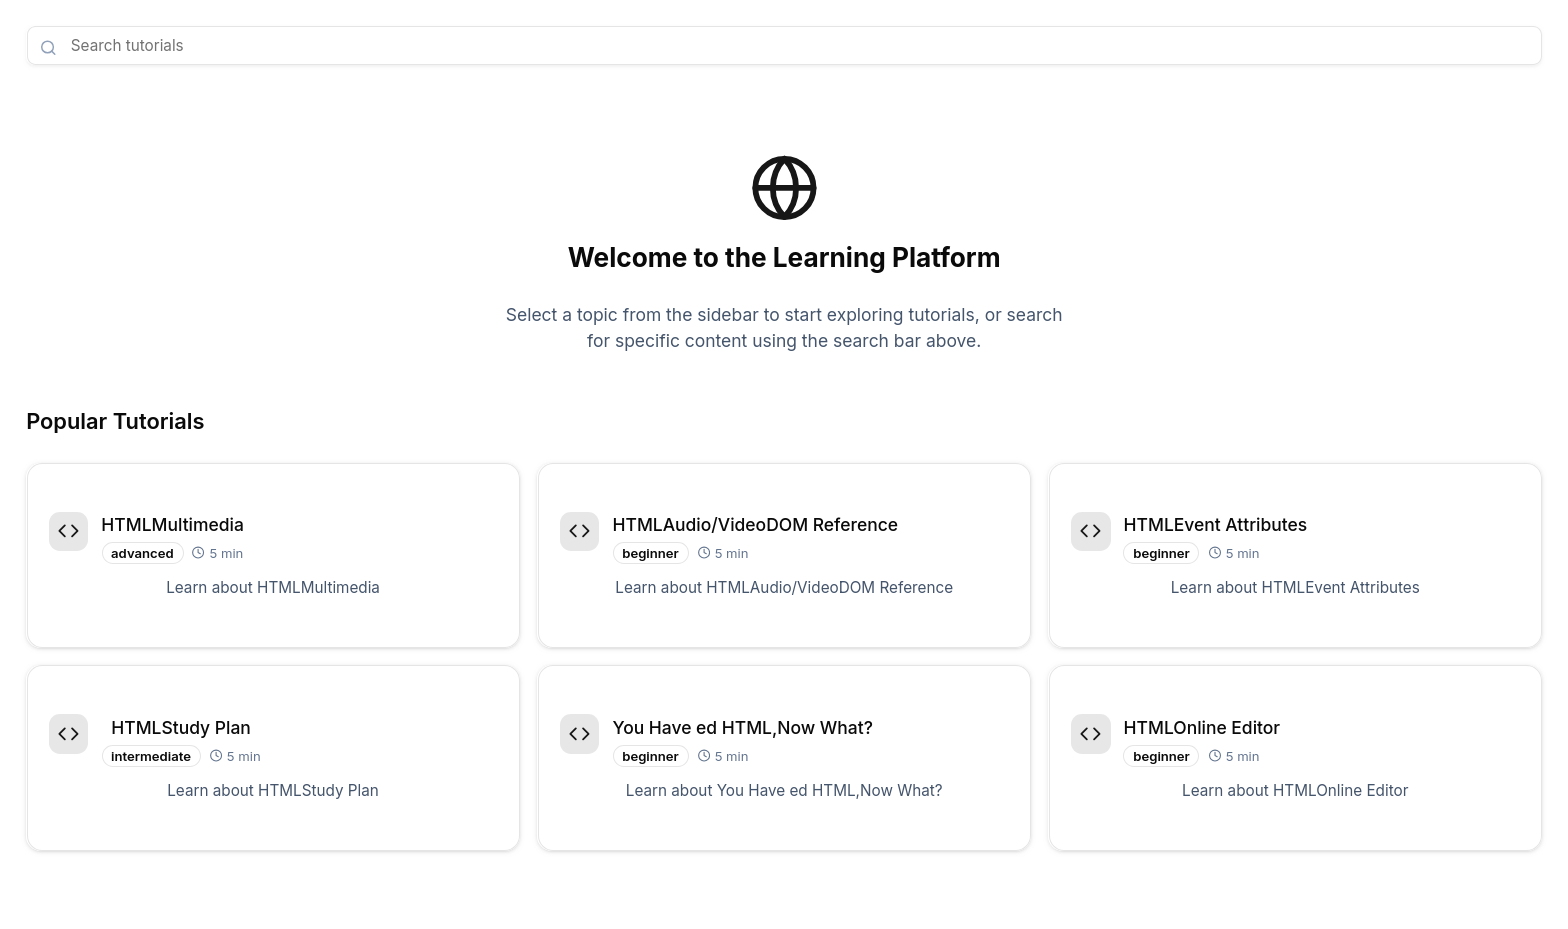
\includegraphics[width=0.9\textwidth]{accueil.png} % REPLACE image (1).png with your main page/tutorials image filename
  \caption{Affichage dynamique des cours sur la page d'accueil, alimenté par les données JSON locales.}
  \label{fig:dynamic_courses_json}
\end{figure}

\begin{figure}[htbp]
  \centering
  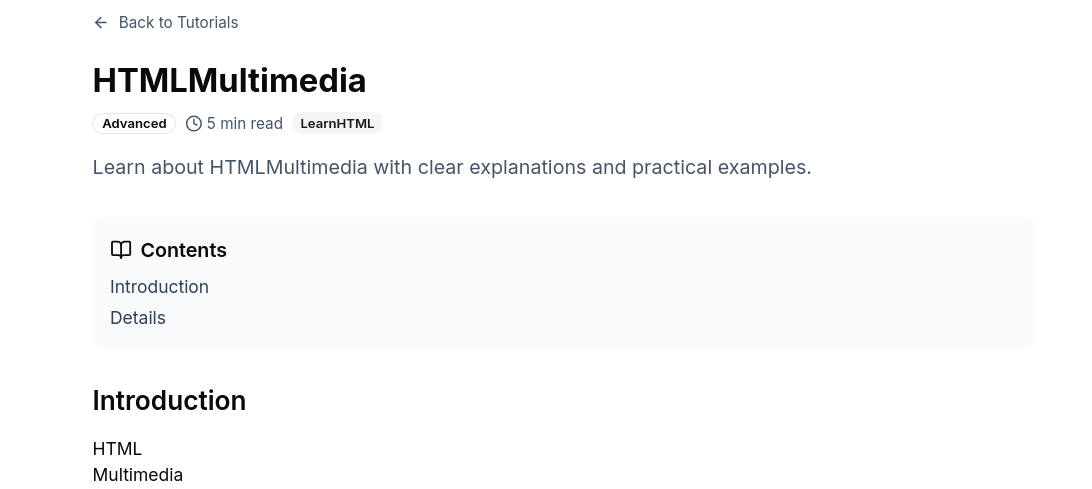
\includegraphics[width=0.9\textwidth]{part1.png} 
   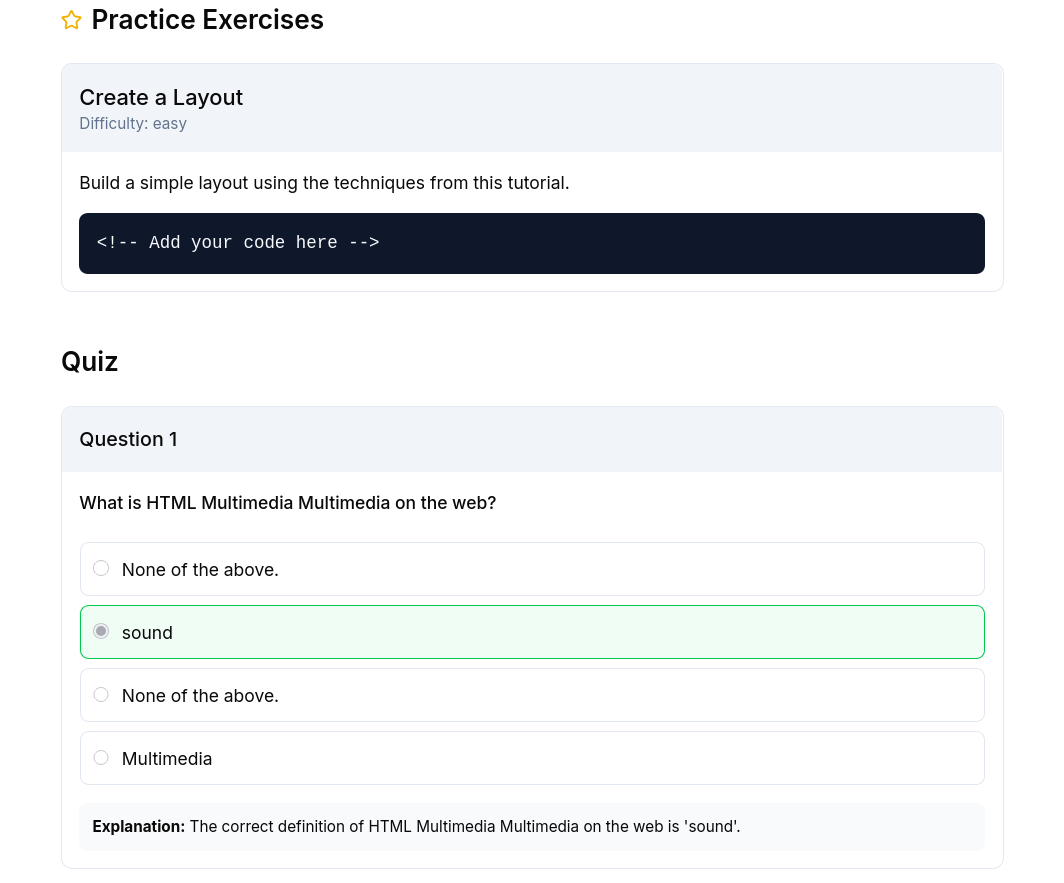
\includegraphics[width=0.9\textwidth]{part2.png} % 
  \caption{Page de détail d'un cours, affichant les informations chargées à partir d'un fichier JSON.}
  \label{fig:course_details_json}
\end{figure}

\subsection{Avantages de l'Approche JSON et Améliorations UI/UX}
Le passage à une gestion des données basée sur des fichiers JSON locaux présente plusieurs avantages significatifs pour le projet :
\begin{itemize}
  \item \textbf{Réduction de la complexité :} Élimination de la nécessité de configurer, gérer et interroger une base de données externe pour le contenu principal.
  \item \textbf{Amélioration de l'expérience développeur (DX) :} Les données sont directement accessibles et modifiables dans des fichiers, ce qui simplifie le développement et le débogage.
  \item \textbf{Facilité de maintenance et d'évolution :} Le code base devient plus simple à appréhender, facilitant les modifications futures et la collaboration.
  \item \textbf{Potentiel d'amélioration des performances :} Grâce aux capacités de rendu côté serveur (SSR) de Next.js et à la lecture directe des fichiers locaux, les temps de chargement peuvent être réduits, surtout pour la récupération initiale des données.
\end{itemize}
Parallèlement à ces changements structurels, des améliorations mineures ont été apportées à l'interface utilisateur (UI) et à l'expérience utilisateur (UX) pour rendre la navigation plus intuitive et la plateforme plus simple à comprendre.

\subsection{Planification pour Demain (Jeudi 22 Mai 2025)} % Updated day and date
La journée de demain sera consacrée à l'enrichissement des fonctionnalités et à l'optimisation de la plateforme :
\begin{itemize}
  \item Se concentrer sur le style manquant, en particulier dans la section des détails des cours pour une présentation plus soignée.
  \item Intégrer un éditeur de code direct dans les pages de tutoriels pour permettre une expérience d'apprentissage interactive.
  \item Améliorer l'interactivité générale de la plateforme, en explorant des animations ou des transitions fluides.
  \item Analyser et implémenter le chargement paresseux (lazy loading) pour les images et potentiellement pour les composants de cours, afin d'optimiser davantage les performances de chargement initial et l'utilisation des ressources.
\end{itemize}

\section{Conclusion}
Cette troisième journée de la troisième semaine a été marquée par une réorientation technique réussie vers l'utilisation de fichiers JSON locaux pour la gestion des données. Cette approche a permis de rendre l'application rapidement et entièrement fonctionnelle pour la récupération et l'affichage du contenu des cours, y compris une barre latérale dynamique. Les avantages en termes de simplification du développement, de maintenance et de potentiel de performance sont notables. Les prochaines étapes se concentreront sur l'amélioration de l'expérience utilisateur, l'intégration de fonctionnalités interactives et l'optimisation continue des performances.

\end{document}